\documentclass[12pt, oneside]{article}
              		% See geometry.pdf to learn the layout options. There are lots.
              		\usepackage[margin=1in]{geometry}
\geometry{letterpaper}                   		% ... or a4paper or a5paper or ... 
%\geometry{landscape}                		% Activate for rotated page geometry
%\usepackage[parfill]{parskip}    		% Activate to begin paragraphs with an empty line rather than an indent
\usepackage{graphicx}				% Use pdf, png, jpg, or eps§ with pdflatex; use eps in DVI mode
								% TeX will automatically convert eps --> pdf in pdflatex		
\usepackage{amssymb}
\usepackage{ragged2e}
\usepackage{circuitikz}

\graphicspath{ {pics/} }

%SetFonts

%SetFonts


\title{ECE 3150 Lab 2}
\author{Aalaap Narasipura}
\date{Febuary 26, 2016}							% Activate to display a given date or no date

\begin{document}
\maketitle
\section{Pre-Lab Work}
\textbf{CMOS Logic Inverter}
\begin{center}


\ctikzset{tripoles/mos style/arrows}
\begin{circuitikz}\draw

(0,0,0) node[nmos] (mos) {}
(mos.base) node[anchor=west] {}
(mos.gate) node[anchor=east] {}
(mos.drain) node[anchor=south] {}
(mos.source) node[anchor=north]{}

(0,1,0) node[pmos] (mos2) {}
(mos2.base) node[anchor=west] {}
(mos2.gate) node[anchor=east] {}
(mos2.drain) node[anchor=south] {}
(mos2.source) node[anchor=north]{}

(mos2.source) ++(0,-.25) -- ++(0,-.511)node[]{} to (mos2.base)
(mos.source) ++(0,-.25) -- ++(0,1.029)node[]{} to (mos.base)

(mos2.source) ++(0,-.25) -- ++(0,.5)node[circ]{} node[right]{\(V_{DD}\)}

(mos.drain) ++(0,-.25) -- ++(2,0)node[circ]{} node[right]{\(V_{out}\)}
(mos.drain)  ++(1,-.25) to [C] ($(mos.drain)+(1,-1)$) node [ground] {}

(mos.gate) -- ++(0,1) to (mos2.gate)
to (mos.gate) ++(0,.5) -- ++(-1,0)node[circ]{} node[left]{\(V_{in}\)}

(mos2.drain) ++(0,-.5) to ($(mos2.drain)+(0,-.75)$) node [ground] {}

;\end{circuitikz}
\end{center}
\textbf{a)} $V_{OUT} < V_{IN}-V_{TN}$\\
\textbf{b)} $V_{OUT} > V_{IN}-V_{TN}$\\
\textbf{c)} $V_{IN} < V_{TN}$\\
\textbf{d)} $V_{OUT} > V_{IN}-V_{TP}$\\
\textbf{e)} $V_{OUT} < V_{IN}-V_{TP}$\\
\textbf{f)} $V_{IN} > V_{TP}+V_{DD}$\\
\textbf{g} %\includegraphics[scale=.3]{exp_amp}\\
$V_{DD} = 5.0V $, $V_{TN} = 1.5V$, $V_{TP} = -1.5V$, finally, $k_n=k_p$\\
\begin{center}
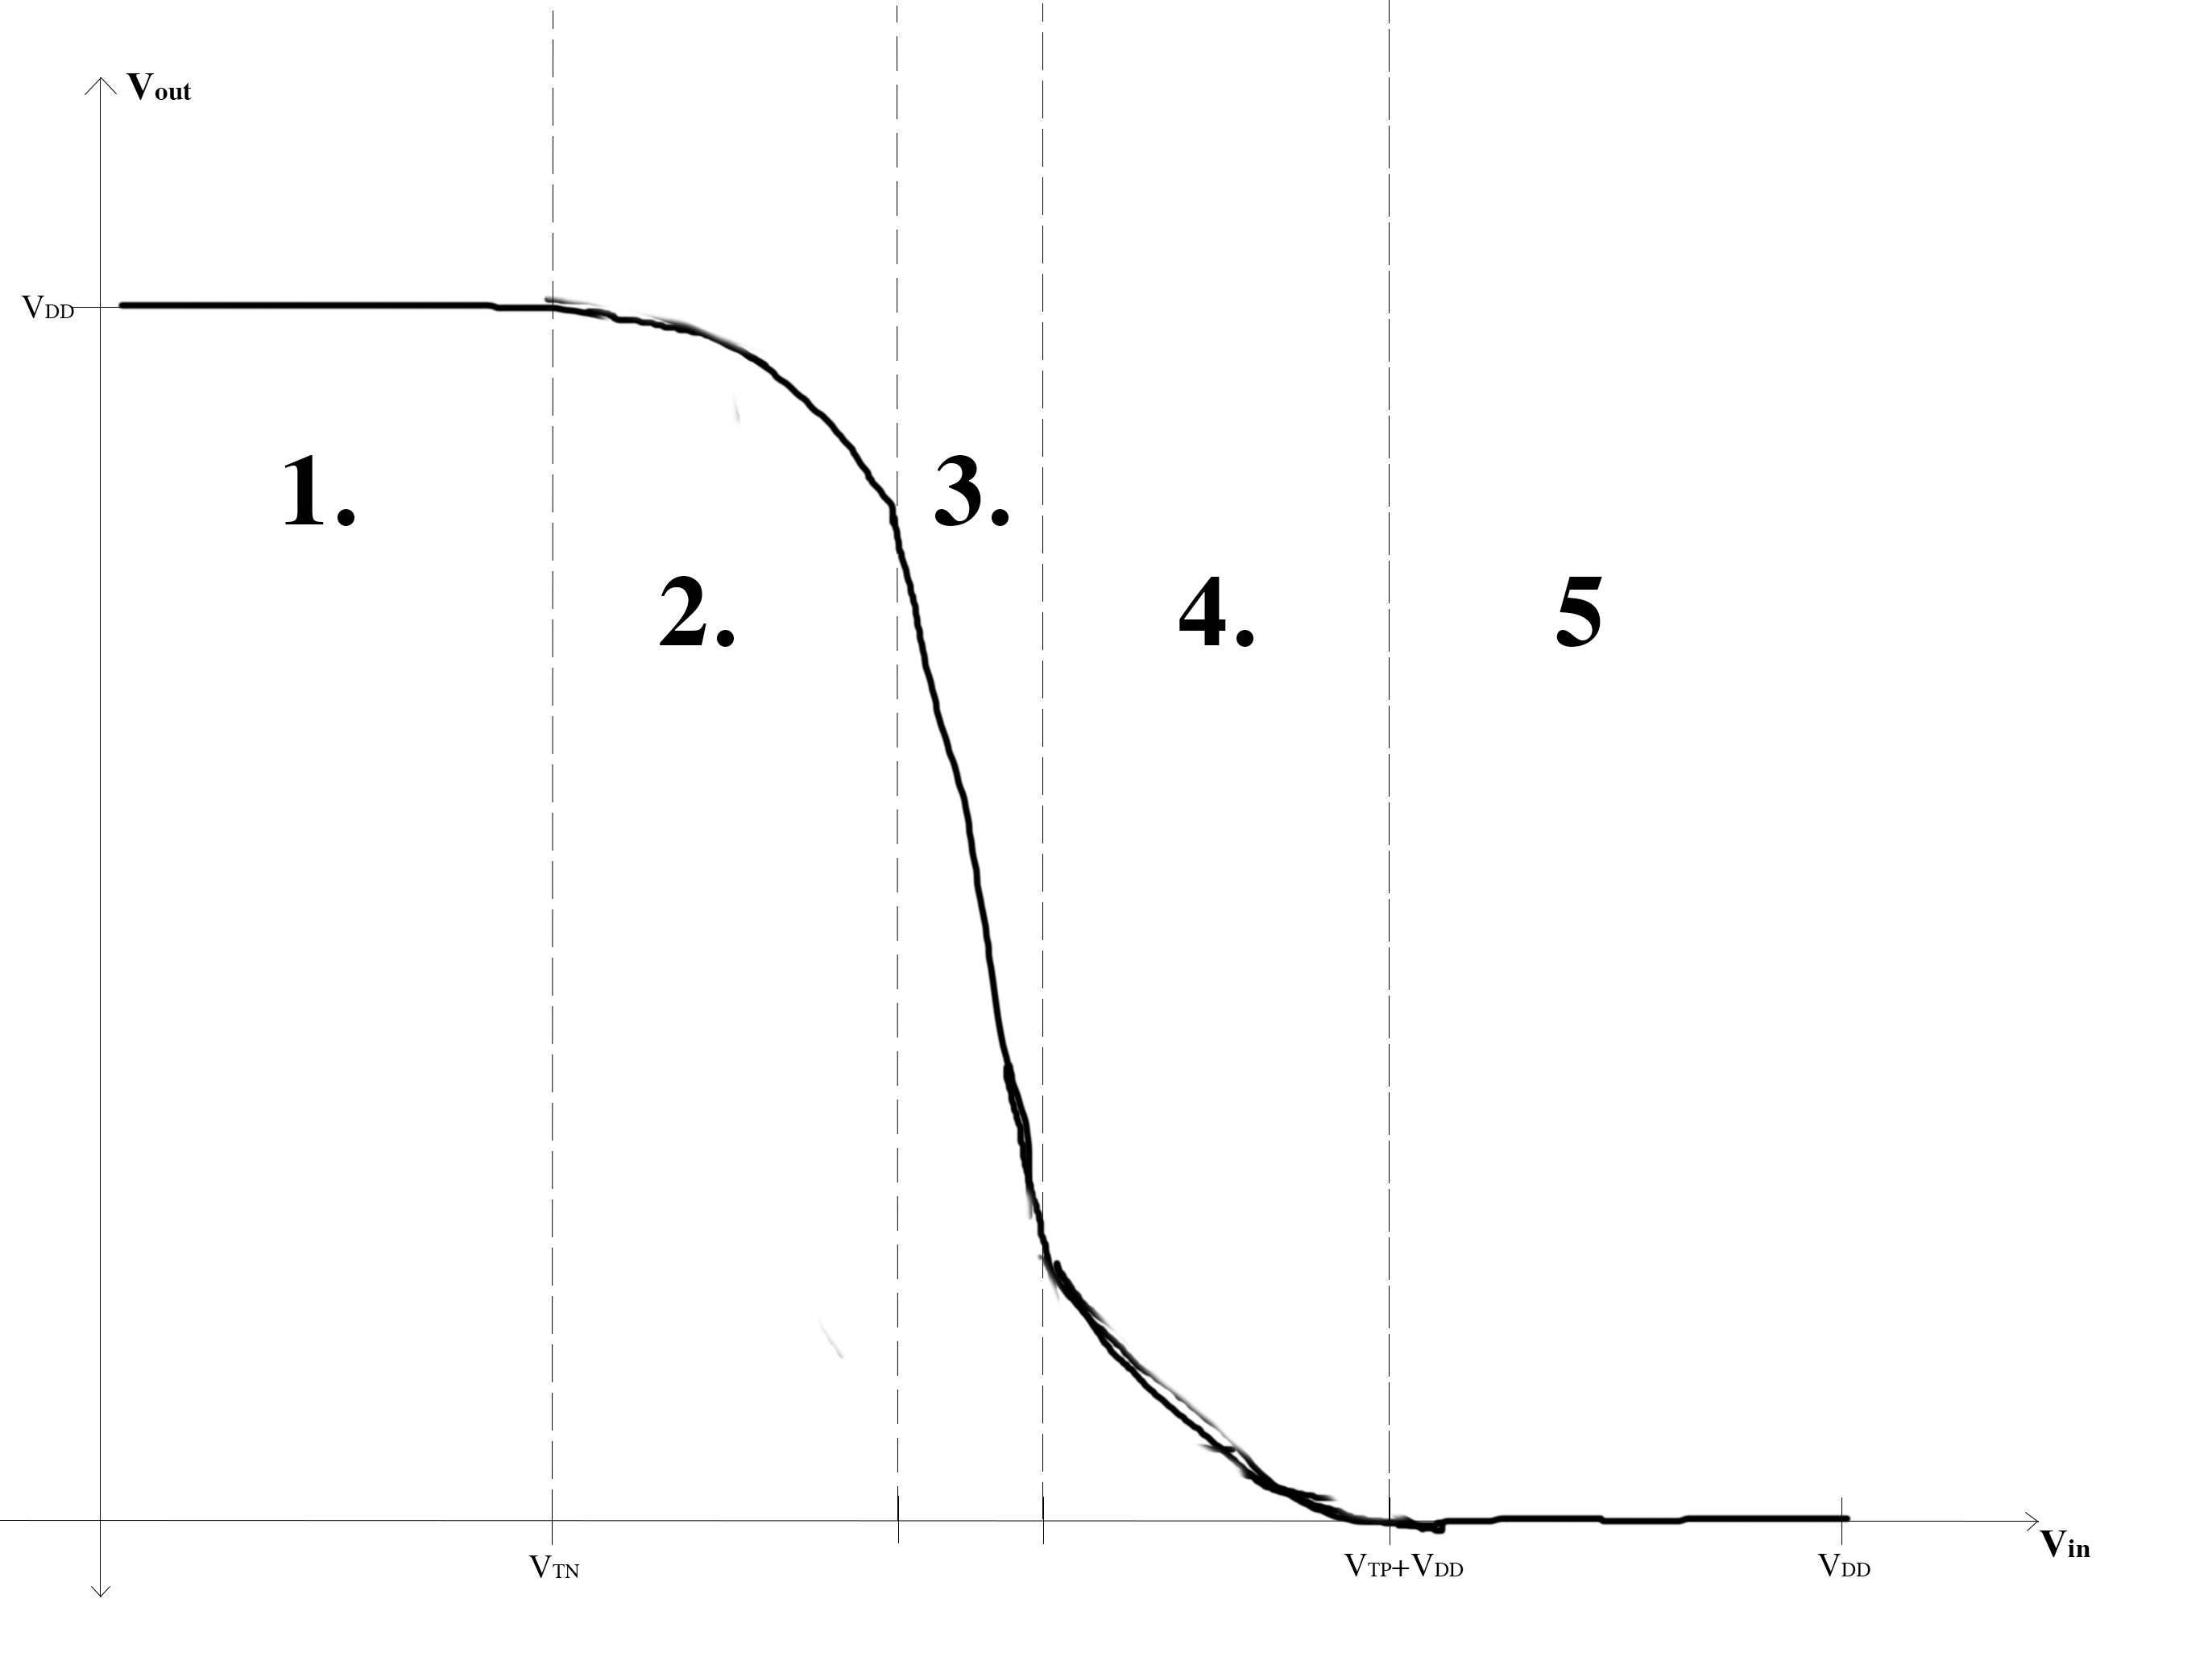
\includegraphics[scale=.1]{part_g}\\
\end{center}
1. NFET in cutoff region, PFET is in linear region\\
2. NFET in saturation region, PFET is in linear region\\
3. Both are in saturation\\
4. NFET in linear region, PFET is in saturation region\\
5. NFET in cutoff linear, PFET is in cutoff region\\
6. This is really cool stuff here

\section{Post Lab Work}
\subsection{Transconductance}
\begin{center}
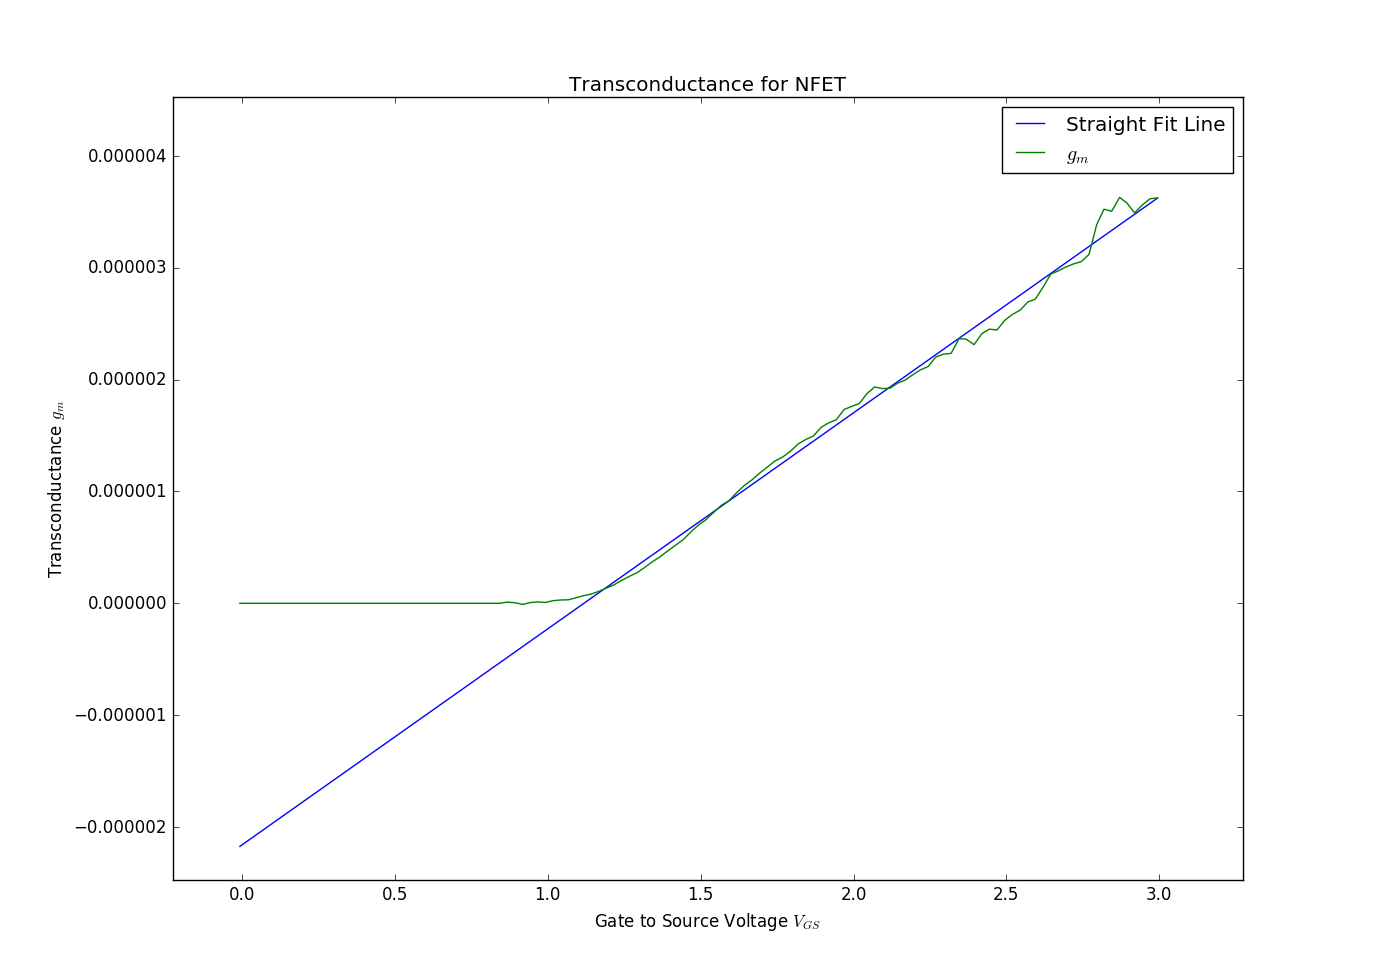
\includegraphics[scale=.35]{nfet_a}\\
Equation of line fit = $y=1.93177*10^{-6}x-2.1607*10^{-6}$\\

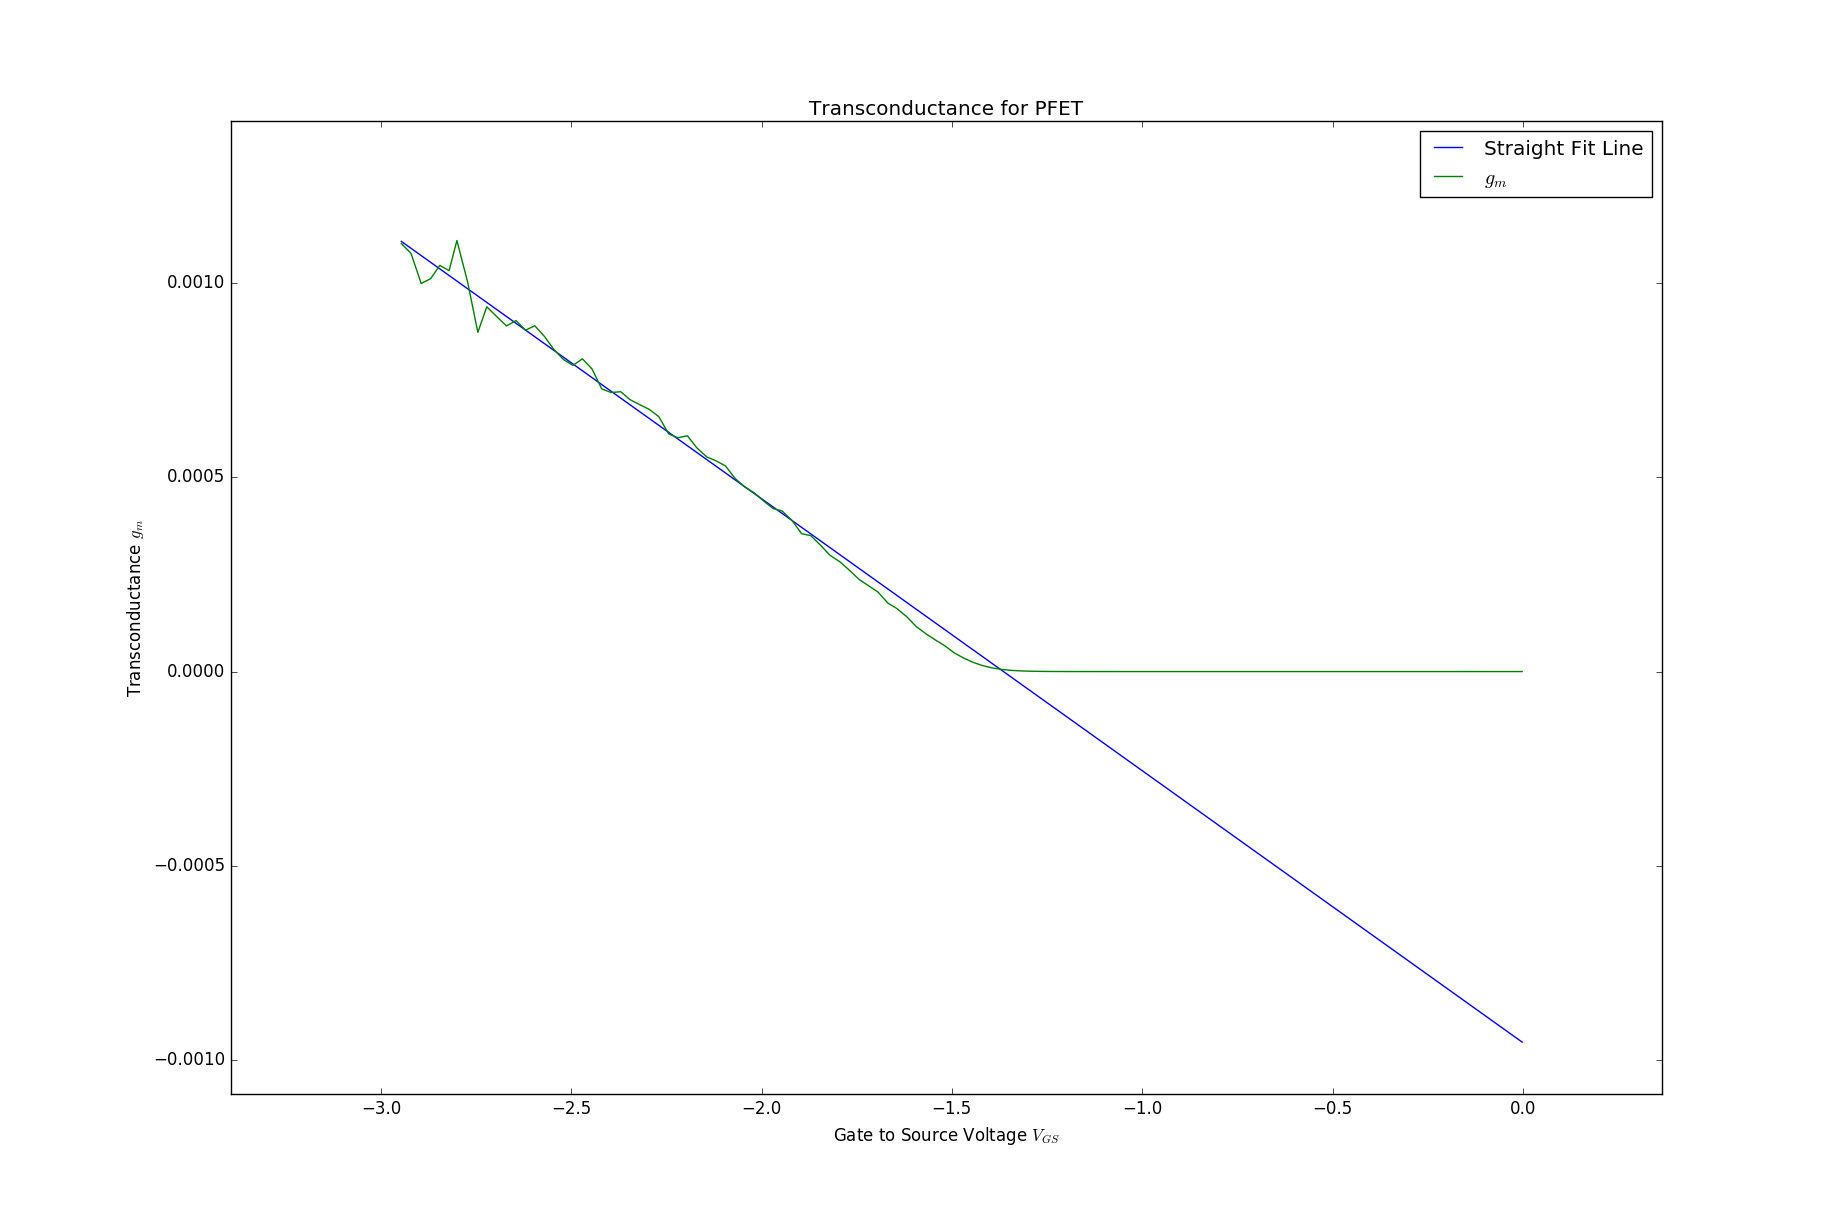
\includegraphics[scale=.35]{pfet_a}\\
Equation of line fit = $y=-.0006996x-.0009546$\\

$V_{tn} = 1.118V$, $k_n= 1.93177*10^{-6} \frac{A}{V^2}$\\
$V_{tp} = -1.42V$, $k_n= -.0006996 \frac{A}{V^2}$\\
The NFET and PFET were not in agreement. I am not entirly sure why the NFET data is so much different. I think that we may have damaged the NFET at some point by having too large of a bias voltage or messing up the sweep voltage. However with this being said, the shape of the curve is what we want. $k_p$ is the correct value based on the transistor data sheet given to us.
\end{center}

\subsection{Subthreshold Condition}
	\begin{center}
		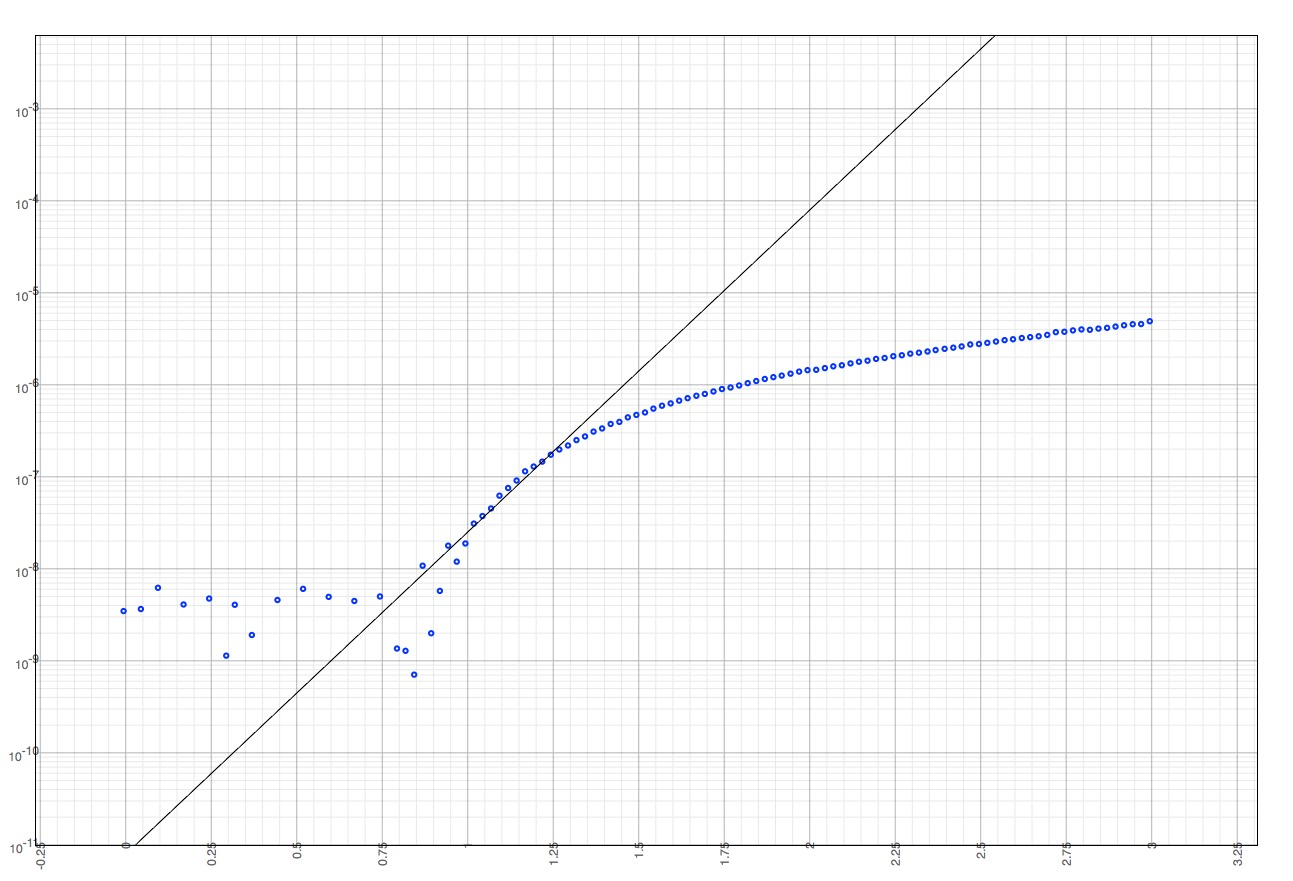
\includegraphics[scale=.4]{NFET_b}\\
		The measured inverse slope value was 175$\frac{mv}{dec}$
	\end{center}

\subsection{FET Output Curves}
	\begin{center}
		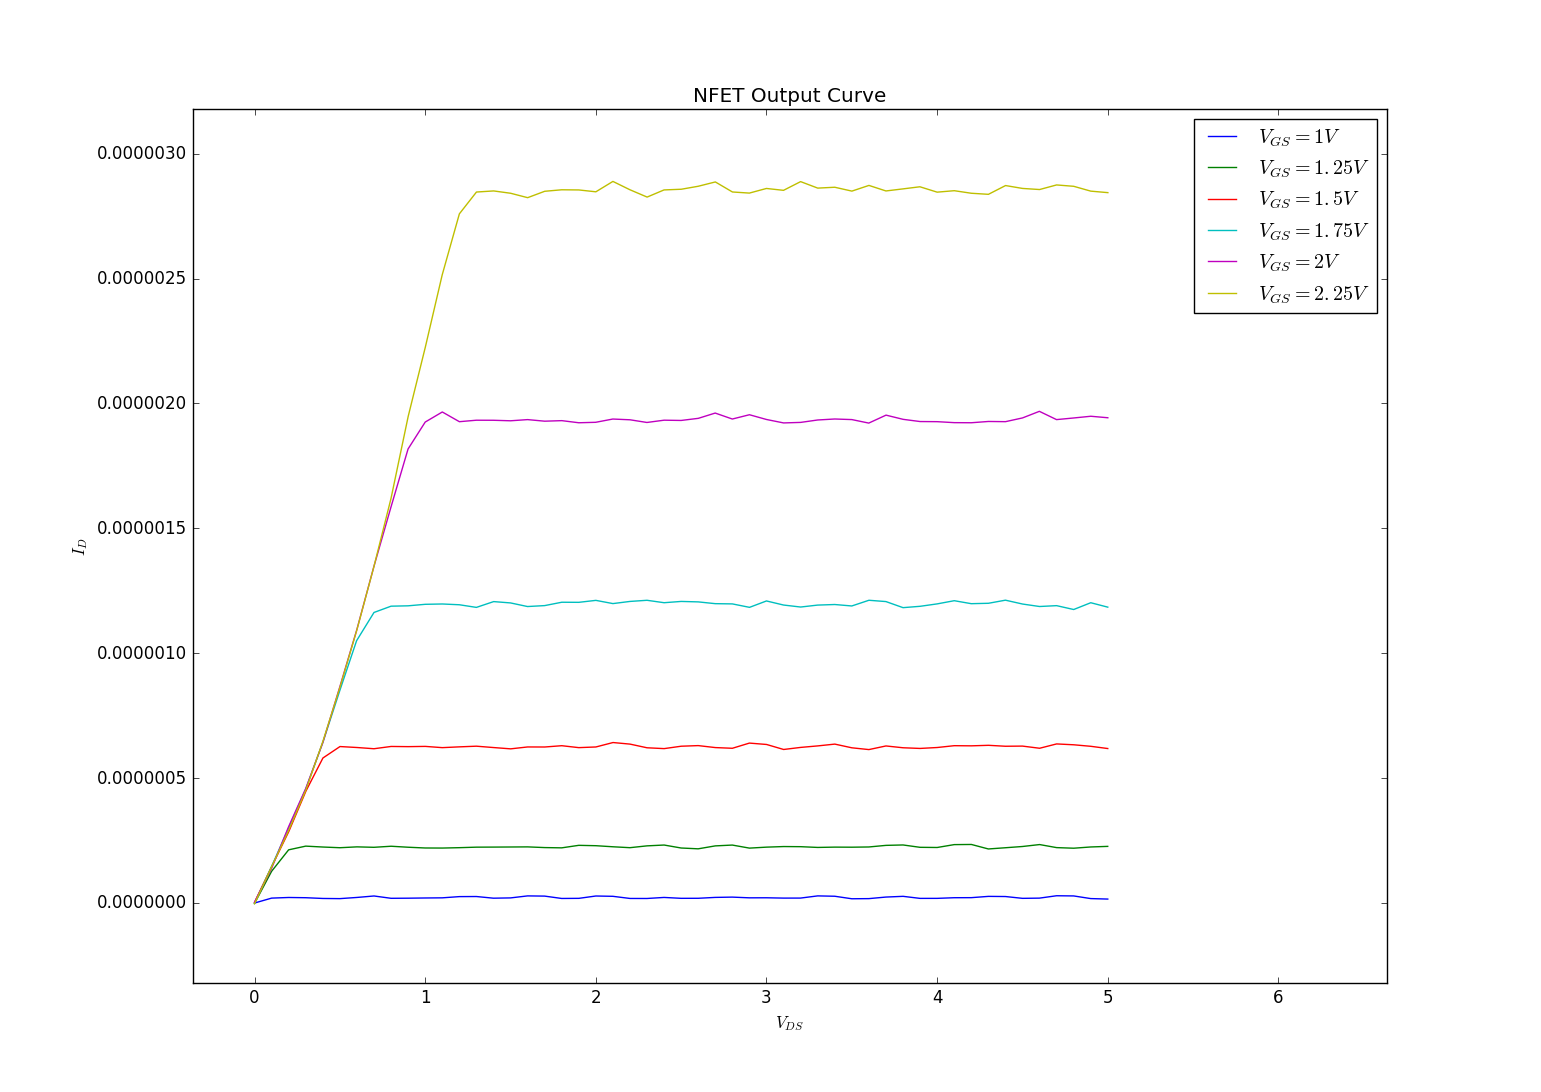
\includegraphics[scale=.35]{nfet_c}\\
		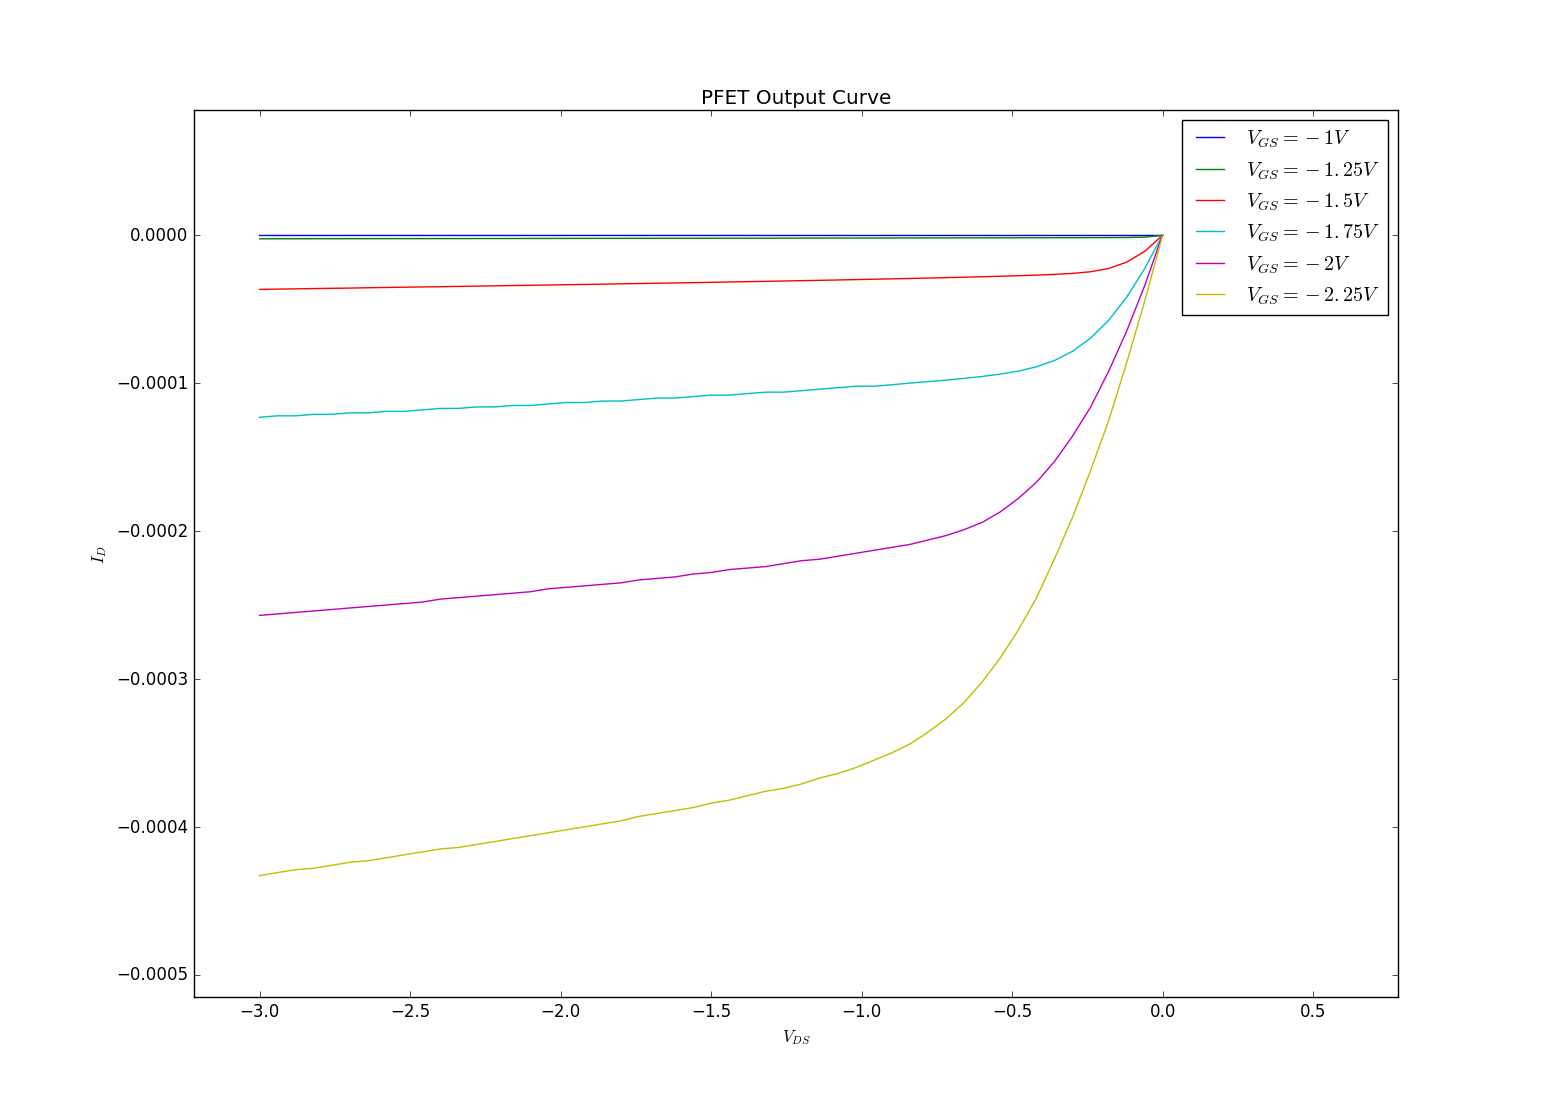
\includegraphics[scale=.4]{pfet_c}\\
		\end{center}
		The slope of the PFET output curve above threshold was larger due tue a larger channel length modulation. The NFET seemingly has a much smaller output current compared to the PFET, but this I believe is due to a damaged NFET. However if you were to scale the NFET data up so it was the same order of magnitude as the PFET it would have larger magnitude output current for a given $V_{GS}$.


\subsection{FET Output Conductance}
	\begin{center}
		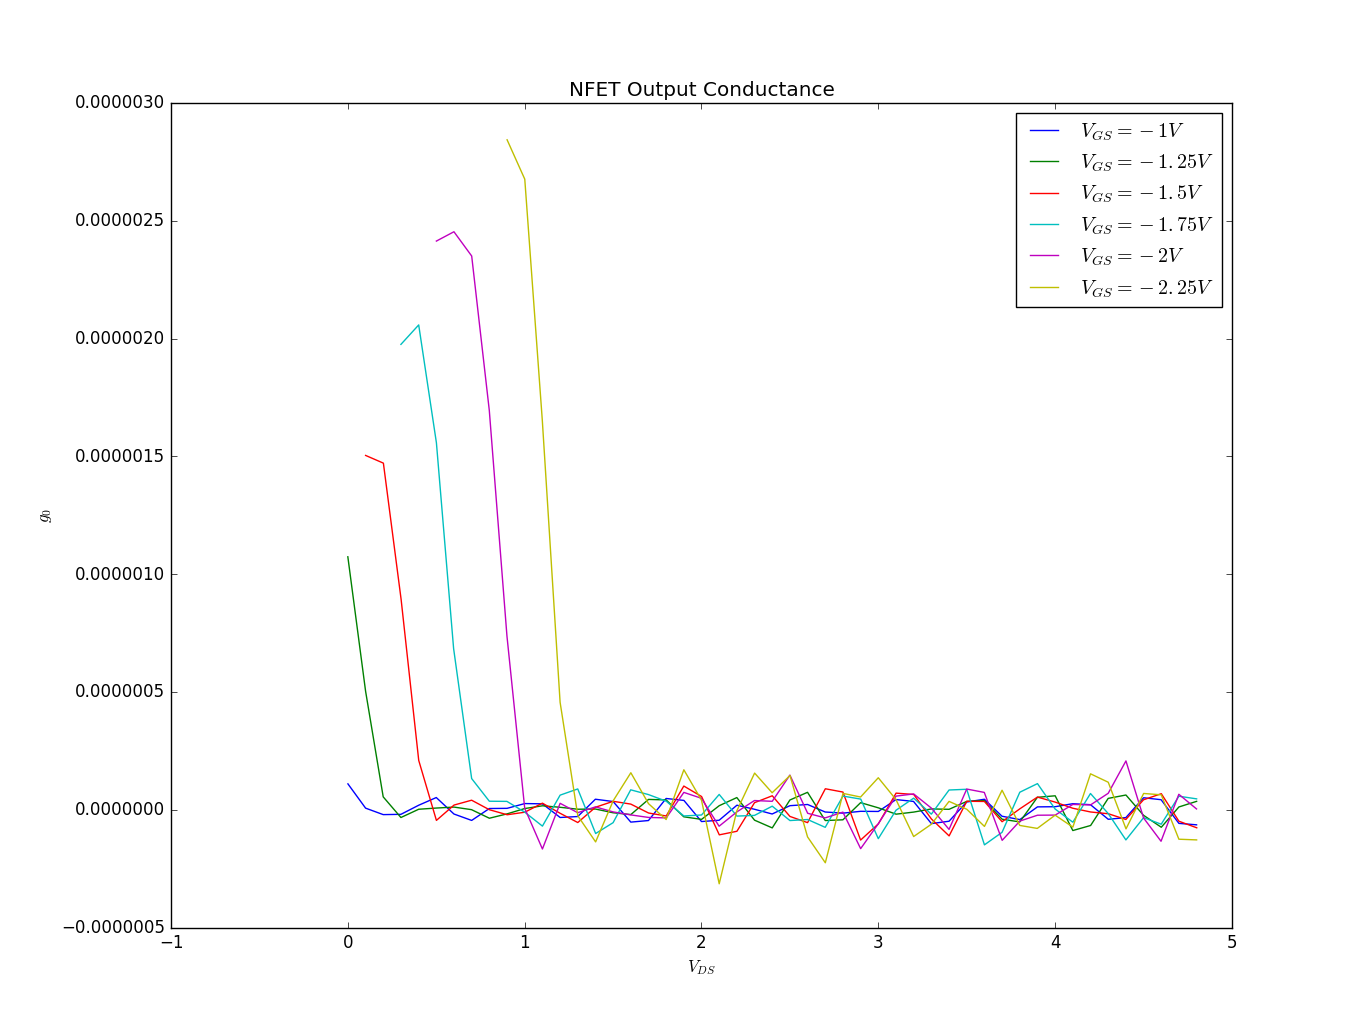
\includegraphics[scale=.4]{nfet_d}\\
		Again the values of $g_o$ we got were quite off when compared to the PFET. We know the PFET is corect because I compared the values we got to the transistor data shet There is also a lot more noise in the NFET data. Both may be due to a damaged NFET. Also I noticed an odd taper down for the NFET.
		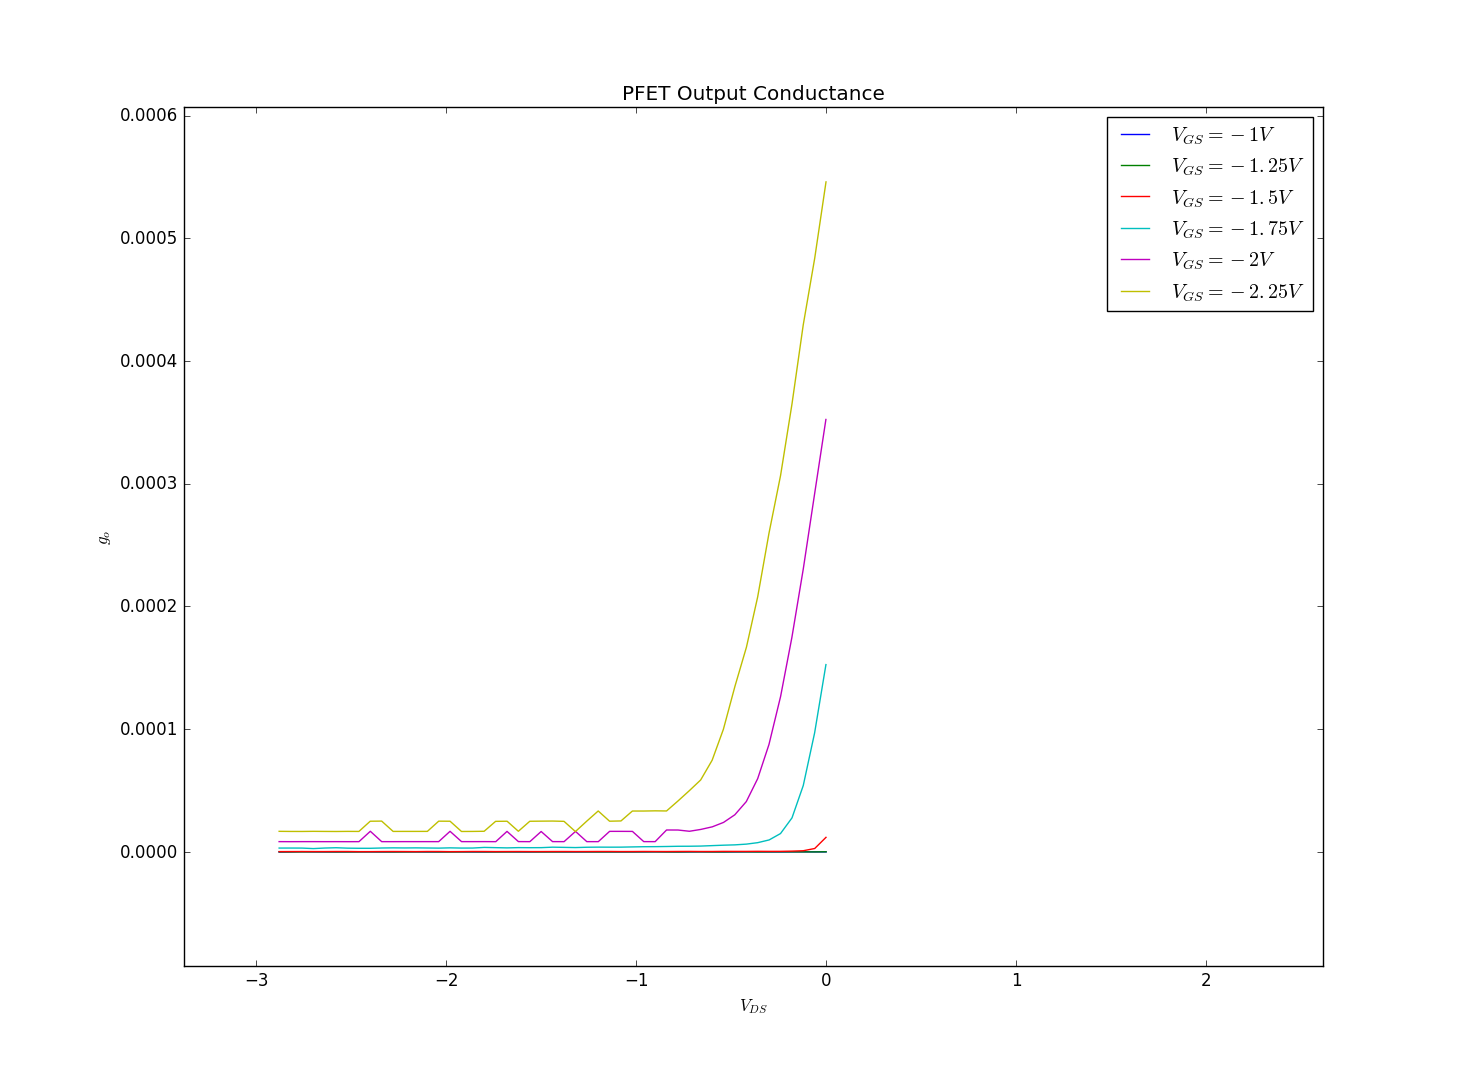
\includegraphics[scale=.4]{pfet_d}\\
		The PFET data shows only up to -3V. However because there will not be much output conductance at voltages less than $V_{TP}$, it can be extrapolated that from -3 V to -5V the data will be very similar if not exact to the values from -2V to -3 V.\\
		I graphed more plots than the post lab said to do because I found it very interesting that at -1V $V_{GS}$ and -1.25V  $V_{GS}$ for the PFET that there was almost no output conductance. A similar thing happened with the NFET for 1V  $V_{GS}$
	\end{center}

\subsection{Diode-Connected NFET}
	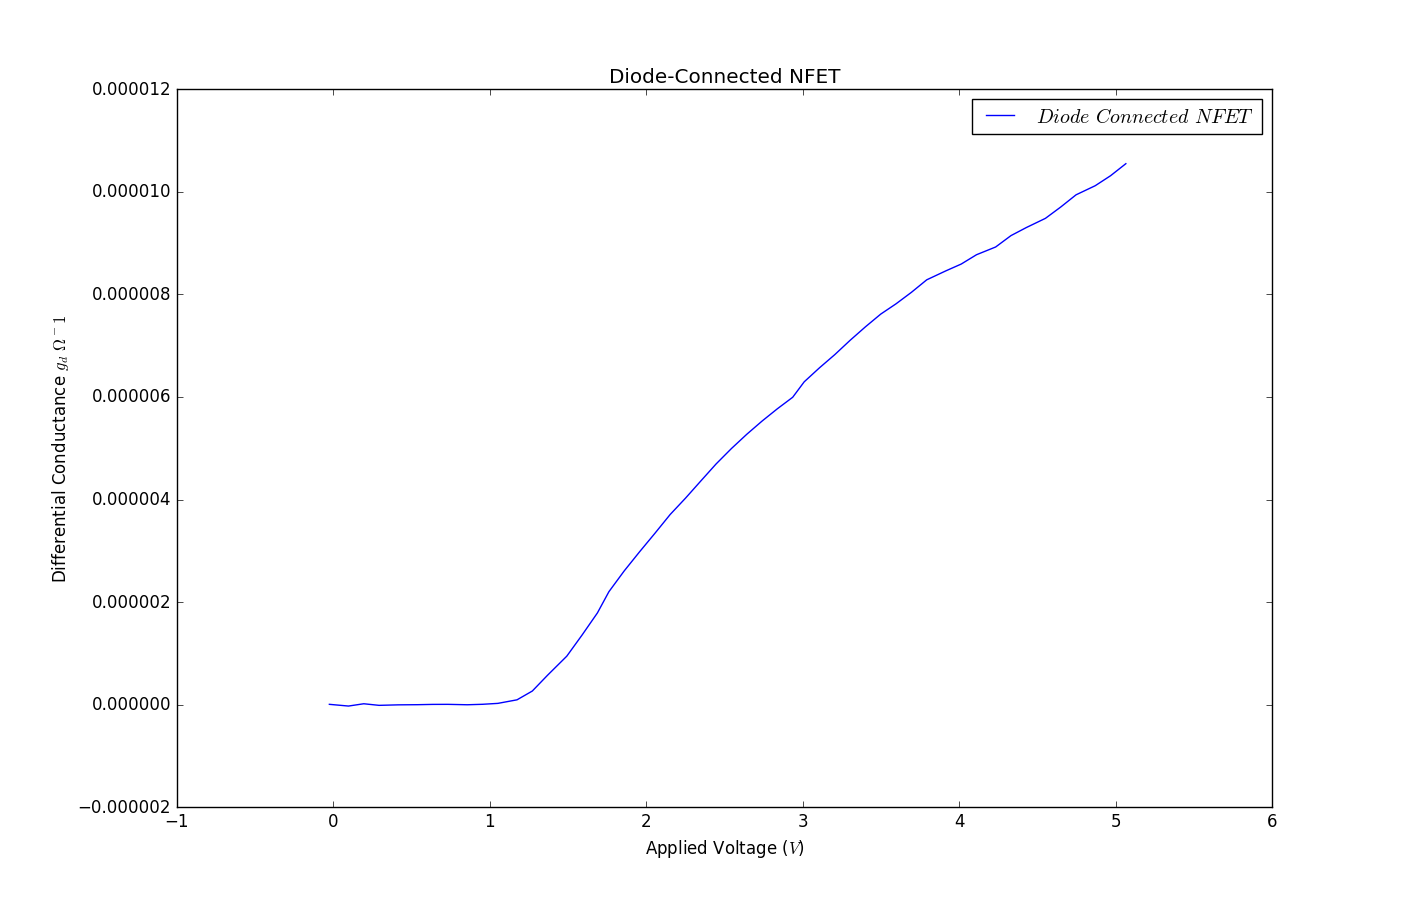
\includegraphics[scale=.4]{figure_1}\\

	The differential conductance that we measured follows the same path as the plot of transconductance in 2.1. The differential conductance bows out away from transconductance plot/ data. However the data values of the Diode-Connected This shows that is only an approximation of the transconductance we measured. It makes sense that these plots are similar because it is still an NFET device.

\subsection{CMOS Inverter}
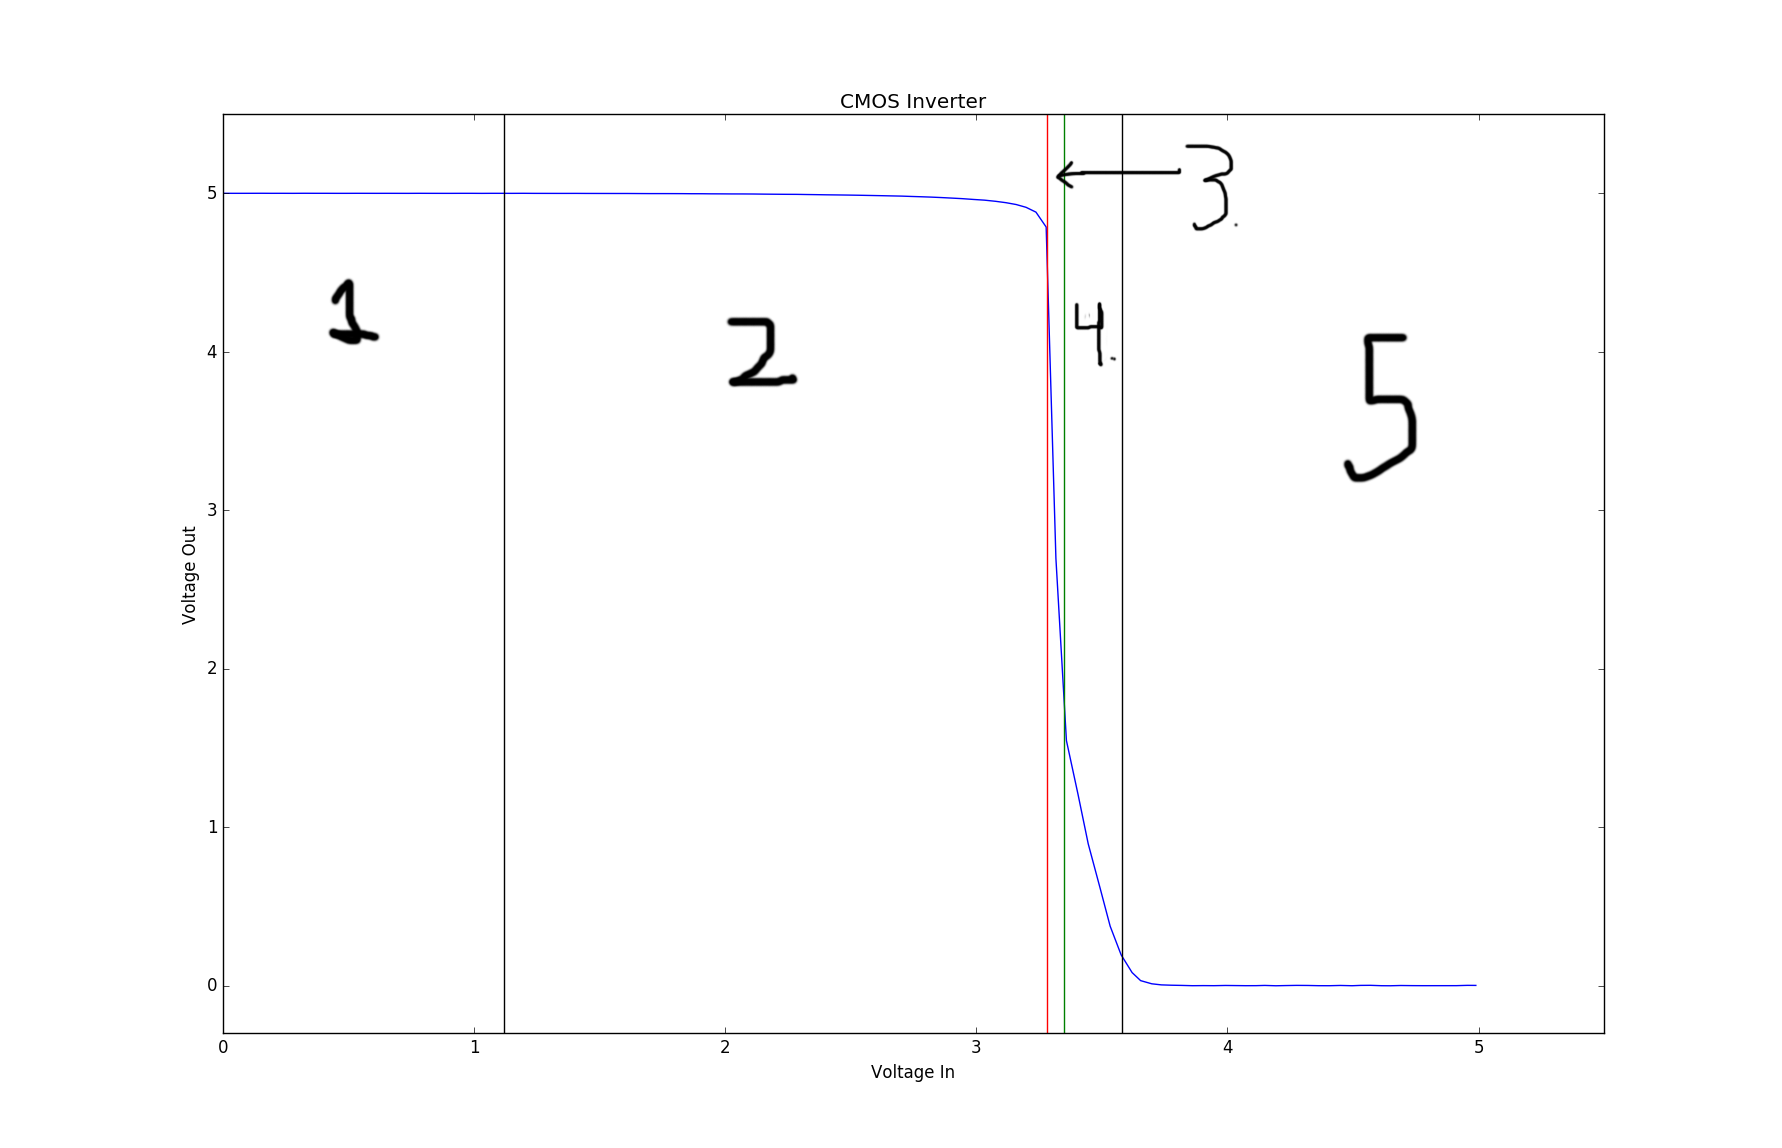
\includegraphics[scale=.3]{inv}\\
1. NFET in cutoff region, PFET is in linear region\\
2. NFET in saturation region, PFET is in linear region\\
3. Both are in saturation\\
4. NFET in linear region, PFET is in saturation region\\
5. NFET in cutoff linear, PFET is in cutoff region\\

Due to the damaged NFET that we have the the CMOS inverter diagram is also incorrect. It again follows the correct shape but the $V_{TN}$ value is very much off.
\end{document}  
